%!TEX root = thesis.tex

\chapter{Breitensuche im invasiven Kontext} % (fold)
\label{cha:breitensuche_im_invasiven_kontext}
In diesem Kapitel wird beschrieben, wie die Breitensuche unter Verwendung des Frameworks invadeX10 implementiert wurde. Aus Zeitgründen konnte in dieser Arbeit nur ein Ansatz herausgearbeitet werden, der noch nicht alle Möglichkeiten des invasiven Rechnens nutzt. Deswegen ist womöglich an einigen Stellen im Algorithmus nicht sofort ersichtlich, weswegen bestimmte Lösungsansätze gewählt wurden. Das liegt daran, dass die Struktur der Implementierungen so gewählt wurde, dass zukünftige Ideen leicht umsetzbar sind.

\section{Unterschiede zum nicht invasiven Fall} % (fold)
\label{sec:unterschiede_zum_nicht_invasiven_fall}
Zunächst seien in diesem Kapitel einige Unterschiede in den Anforderungen und der Problemstellung erläutert. Die Beschreibung der jeweiligen Lösungen finden sich dann in Kapitel \ref{sec:ablauf_des_algorithmus}.

\subsection{Asymmetrie der Rechenleistung} % (fold)
\label{sub:asymmetrie_der_rechenleistung}
Im invasiven Rechnen gibt es das Konzept des Processing Elements (abgekürzt PE). Ein PE ist die abstrakte Repräsentation eines Rechenkerns, auf dem ein Thread ausgeführt werden kann. Jedes PE repräsentiert genau eine Recheneinheit in der Hardware, die in einem bestimmten Bereich liegt. Ein Bereich wird durch gemeinsamen Speicher definiert. Alle Rechenkerne, die sich Speicher teilen, liegen im selben Bereich. Dieser Bereich mit gemeinsamen Speicher wird durch X10 mittels Places abstrahiert. Es kann zum Beispiel ein Prozessor mit 8 Cores vorliegen. Im invadeX10-System existieren dann 8 PEs, die alle auf dem selben Place liegen. Synchronisation und Kommunikation zwischen zwei Activities, die auf dem selben Place laufen, geht wesentlich schneller, was sowohl Bandbreite als auch einmalige Startzeit der Kommunikation betrifft, als wenn die Activities auf unterschiedlichen Places liegen. 

Die Breitensuche wie in Kapitel \ref{sec:1d_partitionierung} löst diese Zweistufigkeit, indem er auf jedem Place gleich viele Daten und damit gleichviel Rechenarbeit legt. Es wird auf jedem Place zunächst genau eine Activity gestartet, sozusagen eine Masteraktivität, die dann zum Beispiel auf Schleifenebene Nebenläufigkeit erzeugt. Es gibt quasi zwei klare Hierarchiestufen der Parallelität. Dieser Ansatz geht davon aus, dass alle Places gleich schnell rechnen, bzw. betrachtet Asymmetrien nicht.

Im invasiven Fall fragt das Programm bei dem Agenten nach Rechenleistung und bekommt daraufhin eine gewisse Menge an PEs als Antwort zurück. Selbst wenn durch Constraints festgelegt würde, dass die PEs gleichmäßig auf Places verteilt sein sollen, kann der Agent das in Abhängigkeit der aktuellen Situation des Gesamtsystems nicht garantieren. Wird der Agent gezwungen, gleichviel Rechenleistung auf jedem Place zu reservieren, liegt womöglich Rechenleistung brach. Deswegen kann sich das Programm nicht darauf verlassen, dass die PEs gleichmäßig über Places verteilt sind. Das Programm findet sich also in der Situation, dass es beispielsweise drei PEs, eine auf Place 0 und zwei auf Place 3 hat. Die erste, intuitive Konsequenz muss sein, dass auf Place 3 doppelt so viele Daten wie auf Place 0 liegen. Im Falle der Breitensuche werden Place 3 also doppelt so viele Knoten gehören wie Place 0. Wird nun ein infect auf die drei PEs aufgerufen, werden korrekterweise drei Activities gestartet, die alle denselben Code ausführen. Allerdings stehen die zwei Activities, die auf dem selben Place laufen, in einem anderen Verhältnis zueinander, als zwei Activities, die auf verschiedenen Places laufen. Die Activities haben für die folgenden Erläuterungen die Nummern 0,1 und 2, wobei Activity 0 auf Place 0 und entsprechen 1 und 2 auf Place 3 liegen.

\begin{itemize}
	\item Will Activity 0 Daten an 1 und 2 schicken, so ist es effizienter diese in einem Kommunikationsvorgang zusammenzufassen, als das IPC-System zweimal zu starten.
	\item Ebenso sollten Activity 1 und 2 gemeinsam ihre Daten an Activity 0 schicken, statt zwei IPC-Vorgänge auszuführen.
\end{itemize}
% subsubsection asymmetrie_der_rechenleistung (end)
Eine Activity muss also den gesamten Kontext kennen und wissen, ob und in welchem Fall sie sich mit anderen Activities auf dem selben Place zusammen tun sollte und wann nicht. Dies wird dadurch erschwert, dass alle Aktivities gleichberechtigt sind. Es gibt also keine \enquote{zentrale Anlaufstelle} für Synchronisation und Kommunikation pro Place.

\subsection{Dynamische Ressourcenverwaltung und Verteilung der Daten} % (fold)
\label{sub:dynamische_ressourcenverwaltung}
Hier ist prinzipiell ein Designentscheidung zu treffen, die nur ein Kompromiss sein kann, da sich zumindest bei der Breitensuche nur schwer folgende Ziele vereinbaren lassen:
\begin{itemize}
	\item Dynamisches invade und retreat je nach benötigter Rechenleistung um nicht benötigte Ressourcen für Andere freizugeben
	\item Daten derart verteilen, dass die Rechenleistung ideal ausgenutzt wird.
\end{itemize}
\underline{Erklärung:} Die Situation sei wie in \ref{sub:asymmetrie_der_rechenleistung}, ein PE auf Place 0, zwei PEs auf Place 3. Es sei bereits eine Iteration der Breitensuche abgeschlossen. Nun ist bekannt, wie viele der Knoten, die auf Place 0 liegen, aktiv sind und wieviel Knoten, die auf Place 3 liegen, aktiv sind. Die Situation sei so, dass beide ungefähr gleich viele Knoten in der nächsten Iteration zu bearbeiten haben, obwohl Place 3 ja die doppelte Menge an Knoten besitzt, also doppelt so viele Knoten potentiell aktiv sein könnten. Die doppelte Rechenleistung auf Place 3 ist damit in der nächsten Iteration nicht zu gebrauchen, da die beiden Activities auf Place 3 nach Beendigung der nächsten Iteration auf Place 0 warten müssten, der für die selbe Iteration ungefähr doppelt so lange benötigen wird. Eine ressourcengewahres System würde also eine der beiden PEs auf Place 3 abgeben. Damit stünde auf den beiden Places gleichviel Rechenleistung zu Verfügung. Durchschnittlich ist die Liste der aktiven Knoten auf Place 3 aber doppelt so lang wie die Liste auf Place 0. Es ist sehr wahrscheinlich und es wird in der Praxis passieren, dass die Liste der aktiven Knoten auf Place 3 wieder deutlich länger wird, als auf Place 0. Das heißt, es ist zu erwarten, dass genau die abgegebene Rechenleistung später wieder gebraucht wird. Die Anwendung kann nun versuchen zu reagieren, indem sie probiert, wieder eine weitere PE auf Place 3 zu bekommen. Allerdings könnten bereits alle anderen PEs auf Place 3 von anderen Anwendung besetzt sein. Zudem entspricht es nicht exakt dem Paradigma des invasiven Rechnens, dem Agenten mitteilen zu müssen, welche PE genau gewünscht ist.

Die naheliegende Antwort auf dieses Problem ist die dynamische Umverteilung der Daten, so dass gleich viele Daten auf Place 0 und 3 liegen, zumindest bis die gewünschte PE wieder verfügbar ist. Dieser Ansatz wurde im Rahmen dieser Arbeit nicht betrachtet, da er zum einen sehr aufwendig zu implementieren ist und zum anderen zu erwarten ist, dass die Performance sehr schlecht ist. Es müssten große Datenmengen (Adjazenzlisten, Distanzarrays) verschickt werden, größere Arrays alloziert werden, usw.

Zusammenfassend kann man sagen, dass ein Algorithmus, der auf partitionierten Daten (ein Graph bei BFS) arbeitet, nur sehr schwierig gleichzeitig temporär ungenutzte Ressourcen abgeben und trotzdem noch maximal effizient arbeiten kann. In dieser Arbeit entspricht zwar jede BFS-Iteration einem \textit{invade}, allerdings werden zwischen den Iterationen keine Ressourcen abgegeben oder angefordert.
% subsubsection dynamische_ressourcenverwaltung (end)

\subsection{Nicht fortlaufende Indizes} % (fold)
\label{ssub:nicht_fortlaufende_indizes}
Trotz Verwendung des InvaIC Frameworks, soll die X10 API weiter genutzt werden können. Die X10-Funktionalitäten rund um Distributions und DistArrays arbeitet auf der Basis von Places und deren Nummerierung. Aus diesem Grund kann man im invasiven Fall nicht komplett von der Vorstellung von Places weggehen, sondern muss im Auge behalten, auf welchem Place welche Daten liegen. Im reinen X10 sind die Places immer von 0 bis p-1 (bei p Places) durchnummeriert. Das macht die Nummer eines Places zu einem sehr praktischen Ausgangspunkt, um mit Indizes zu rechnen. Es kann zum Beispiel ein DistArray der Größe p erstellt werden, wenn auf jedem Place genau ein Datum liegen soll und jeder Place kann mit seinem eigenen Index auf seine eigenen Daten zugreifen.

Im invasiven Fall werden vom Agent zunächst nur ProcessingElements bereitgestellt. Auf welchem Place diese liegen, ist für den Klienten nur bedingt beeinflussbar, sofern er nicht bereit ist auf Rechenleistung zu verzichten. Dadurch ist keine natürliche Nummerierung der Places mehr vorhanden. Es lässt sich nicht vermeiden, etwas Speicherplatz und Rechenleistung zu benutzen, um dieses Problem zu lösen. Der unten stehende Vergleich des Codes zum Feststellen, welcher der besitzende Place von Knoten k ist, verdeutlicht das Problem. $p$ ist die Anzahl an Places, \textit{placesList} eine Liste aller Places und \textit{mapNodeToPlaceIndex} ein Funktion. Damit die zweite Berechnung funktioniert, muss vorher schon eine Datenstruktur mit dem vollständigen wissen über alle PEs initialisiert worden sein.
\begin{algorithm}
	\caption{Durchnummerierter Fall, wie in Kapitel \ref{sec:1d_partitionierung}}
	\label{alg:owner_consecutive}
	\begin{algorithmic}[1]
		\State \textbf{val} owner = k / p
	\end{algorithmic}
\end{algorithm}

\begin{algorithm}
	\caption{Nicht durchnummerierter Fall, wie in diesem Kapitel}
	\label{alg:owner_random}
	\begin{algorithmic}[1]
		\State \textbf{val} ownerId = mapNodeToPlaceIndex(k) // Position des owners in der placesList
		\State \textbf{val} owner   = placesList[ownerId]
	\end{algorithmic}
\end{algorithm}
% subsubsection nicht_fortlaufende_indizes (end)

Das Problem wurde gelöst, indem mit eine Art virtuelle Placesverwaltung eingeführt wurde. Direkt nachdem bekannt ist, welche PEs zur Verfügung stehen, werden alle Places in einer Liste sortiert. Ab diesem Zeitpunkt wird ausschließlich mit dem Rang des Places in der sortierten Liste gerechnet. Die Ränge sind durchnummeriert von 0 bis p-1, womit die gewünscht Situation hergestellt ist. Die einzige Stelle, an der wieder das ursprüngliche Placeobjekt verwendet werden muss, ist beim Argument eines at{}-Blocks. Der Zugriff geht  über den Index in konstanter Zeit.

% subsection unterschiede_zum_nicht_invasiven_fall (end)
\section{Ablauf des Algorithmus} % (fold)
\label{sec:ablauf_des_algorithmus}
Aus Zeitmangel wurde im Rahmen dieser Arbeit die Breitensuche im invasiven Fall nur mittels der 1D-Dekomposition implementiert. Grundsätzlich ist der Algorithmus implementiert, wie er in Kapitel \ref{sec:1d_partitionierung} beschrieben wurde. In diesem Kapitel werden deswegen in erster Linie die gewählten Lösungsansätze zu den Problem aus Kapitel \ref{sec:unterschiede_zum_nicht_invasiven_fall} beschrieben.
\begin{figure}[ht]
	\centering
	\label{img:invasive-flow}
	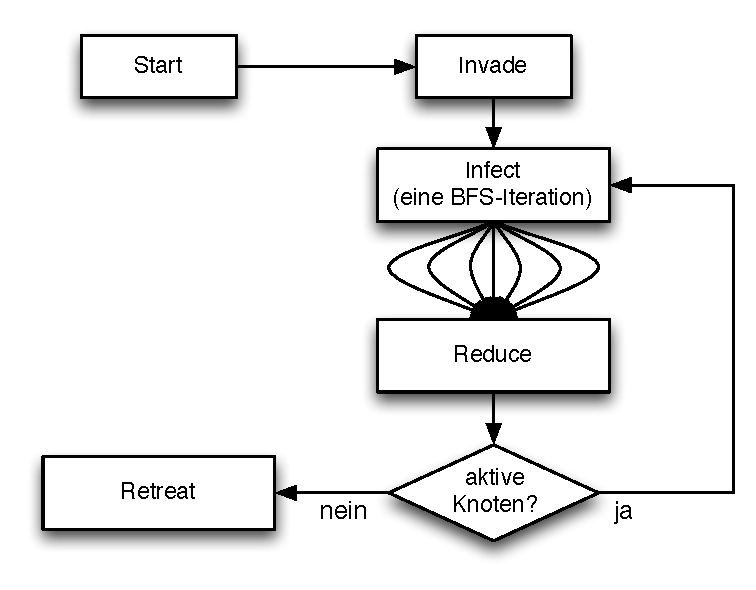
\includegraphics{pics/invasive-flow.pdf}
	\caption{Grundsätzlicher Ablauf der Breitensuche. Zu beachten ist, dass zwischen den einzelnen Iterationen kein \textit{retreat} und kein invade stattfindet.}
\end{figure}

\subsection{Dekomposition und Datenhaltung} % (fold)
\label{sub:dekomposition_und_datenhaltung}

Sobald der Algorithmus nach dem Start den Graph vollständig eingelesen hat und die Antwort des \textit{invade} bekommen hat (eine Liste von PEs), beginnt er damit, sich die benötigten Datenstrukturen aufzubauen.
\begin{itemize}
	\item ProcessingElements nach Placenummer sortieren. Liste alle involvierten Places in eben dieser Reihenfolge aufstellen und zu jedem Place die Anzahl an verfügbaren PEs in ein Array schreiben. An der Stelle 0 in diesem Array steht also, wie viele PEs auf dem Place zur Verfügung stehen, der in der Placeliste an erster Stelle (Index 0) steht.
	\item Die Menge an Knoten wird so unterteilt, dass jede PE ein gleichgroßen Teil bekommt. Wichtig ist, dass alle PEs, die auf dem selben Place liegen, benachbarte Intervalle der Knotenliste bekommen. Es wird entsprechend Platz für die Adjazenzlisten auf den Places reserviert. Alle Knoten, die zu einem Place gehören, gehören allen dortigen PEs gemeinsam. Um aufzulösen, welchem Place ein Knoten gehört, wird ein Array berechnet, dass für jede PE (in der Reihenfolge der Liste aus dem ersten Punkt) enthält auf welchem Place sie liegt. Um den Besitzer von Knoten k zu finden, muss so zur Laufzeit nur noch k durch die Anzahl an PEs geteilt werden und das Ergebnis als Index für den Arrayzugriff verwendet werden. Das Ergebnis ist wiederum die Stelle der Placeliste, an der der besitzende Place steht.
	\item Die selbe Initialisierung muss für das DistArray passieren, dass die BFS-Distanzen halten soll.
	\item Es wird pro Place für jeden anderen Place ein Empfangspuffer erstellt. Diese Empfangspuffer befinden sich in einem DistArray mit einer UniqueDist, das bedeutet, dass auf jedem Place genau ein Datum(=Array aus Puffern) liegt.
	\item Es werden pro Place genau soviele Listen für aktive Knoten erstellt, wie es aktive PEs auf diesem Place gibt.
\end{itemize}

% subsubsection dekomposition_und_datenhaltung (end)
\subsection{Zweistufiges Infect und Indizierung} % (fold)
\label{sub:zweistufiges_infect}
Der Algorithmus verwendet die \textit{Clock}-Funktionalität von X10. Eine Clock entspricht einer Barriere, die alle Aktivitäten bei Erreichen so lange blockiert, bis alle registrierten Aktivitäten die Barriere erreicht haben. Es wird sowohl für alle Aktivitäten (es gibt eine Aktivität pro PE) global eine Clock benötigt, als auch lokal zwischen je allen Aktivitäten, die auf dem selben Place liegen. Um diese Clocks zu erstellen, ist es nötig den Infect-Aufruf manuell zweistufig zu implementieren. Zunächst wird die globale Clock erstellt, dann wird eine Aktivität pro involviertem Place gestartet, die sich aber nicht in der Clock registrieren. Anschließend wird von der einen Aktivität auf jedem Place eine weitere Clock erstellt und pro PE, die auf diesem Place zur Verfügung steht eine Aktivität gestartet. Diese Aktivität registriert sich jetzt in beiden oben erstellten Clocks und beginnt mit der BFS.

Ein weiterer Vorteil des zweistufigen Infects ist es, dass sehr einfach jeder Aktivität ein globaler Index und ein lokaler Index zugeteilt werden kann. Der lokale Index ist die Nummer einer Aktivität auf einem Place. Vor allem der lokale Index wird im Weiteren sehr nützlich sein.
% subsubsection zweistufiges_infect (end)

\subsection{Lokale Parallelität} % (fold)
\label{sub:lokale_parallelit_t}
Wie die Kollaboration zwischen den einzelnen Places aussieht wurde bereits in Kapitel \ref{sec:1d_partitionierung} beschrieben. Ein Place als ganzes Verhält sich im invasiven Fall exakt gleich. Allerdings gibt es keine \enquote{Masteraktivity} pro Place, die Jobs verteilen kann und für die Synchronisation sorgt. Stattdessen werden mehrere gleichberechtigte Activities gestartet, die trotzdem auf den selben Daten arbeiten sollen. In diesem Abschnitt wird beschrieben, wie diese Zusammenarbeit gelöst wurde. Dazu werden die Phasen aus Kapitel \ref{sec:1d_partitionierung} aufgegriffen. Eine genaue Beschreibung der einzelnen Phasen findet sich auch dort und wird hier nicht wiederholt. Wichtig ist, dass jede Activity die Information hat, die wievielte von wie vielen sie auf diesem Place ist.

\subsection{Getrennte Puffer für aktive Knoten} % (fold)
\label{sub:getrennte_puffer_f_r_aktive_knoten}
In der hier gewählten Implementierung hält jede PE eine eigene Liste für aktive Knoten. Dadurch hat jede PE exlkusives Schreibrecht in die eigene Liste, was Synchronisation in Phase 3 einspart. Aus dem exklusiven Schreibrecht folgt sofort, dass in Phase 3 mindestens PE nichts zu tun hat, falls es mehr PEs auf ihrem Place gibt, als es insgesamt Places gibt. In diesem Fall ist den PEs mit einer zu hohen Id kein Empfangspuffer zum lesen zugeordnet.
% subsection getrennte_puffer_f_r_aktive_knoten (end)

\subsection{Phase 1: Adjazente Knoten sortieren} % (fold)
\label{sub:phase_1_invasive}
Die Liste der aktiven Knoten für jede PE einmal vorhanden. Es handelt sich dabei um ein Array von Arraylisten, so dass der Zugriff auf ein beliebiges Element einer beliebigen Liste sehr schnell in konstanter Zeit geschehen kann. Zunächst zählt jedes PE zusammen, viewiele Elemente insgesamt in allen Listen liegen, also wieviele aktive Knoten es auf diesem Place gibt. Jedes PE rechnet sich nun aus, welcher Teil der aktiven Knoten, ihr zustehen. Zum Beispiel berechnet PE 0: 5 Elemente ab Index 0 und PE1 3 Elemente ab Index 5. Aus welchen Listen diese Elemente stammen ist zu diesem Zeitpunkt nicht bekannt. Es könnten zum Beispiel alle Elemente in der zweiten Liste liegen. Der Algorithmus, um über alle Elemente zu iterieren, ist in \ref{alg:iterate_active_nodes} beschrieben.

\begin{algorithm}
	\caption{Über mehrere Listen iterieren}
	\label{alg:iterate_active_nodes}
	\begin{algorithmic}[1]
		\State var min : Int // Start Index of Region
		\State var listIndex : Int = 0
		\For{counter $\in$ length-1..0}

			// Skip to the list containing the first element
			\While{min $\le$ activeNodes(listIndex).size}
				\State min -= activeNodes(listIndex).size
				\State listIndex++;
			\EndWhile

			// calculate how many elements to take from current list
			\State val upperBoundForThisList = min(current(listIndex).size(), min + counter);
            \State val elementsTakenFromThisList = upperBoundForThisList - min;
            \State counter -= elementsTakenFromThisList; // if counter < 0, the outer loop ends

            \For{idx=min; idx < upperBoundForThisList; idx++}
            	\State element = activeNodes(listIndex)(idx)
            	\State // Do Stuff
            \EndFor
            \State min = activeNodes(listIndex).size() // The next element is from the next list

		\EndFor
	\end{algorithmic}
\end{algorithm}
Es wird zu jeder Zeit durch den \textit{listIndex} die aktuell akive Liste gespeichert. Die erste while-Schleife springt solange zur nächsten Liste, bis der Index innerhalb der aktuellen Liste ist. Dazu wird in jeder Iteration die Größe der aktuellen Liste von Startindex abgezogen. Wenn der Startindex innerhalb der aktuellen Liste ist, wird while-Schleife verlassen. Danach wird ausgerechnet, wie lange Elemente aus der aktuellen Liste genommen werden. Wenn noch mehr Elemente gebraucht werden, als die Liste lang ist, dann ist die Obergrenze die Listengröße, ansonsten der Startindex + Anzahl an Elementen.

Diese Implementierung gönnt sich pro PE ein Set von Sendepuffern. Ein Set von Sendepuffern besteht aus einem Sendepuffer pro beteiligtem Place. Es gibt also auf Place k $p * c_k$ Sendepuffer, wobei p die Anzahl der Places und $c_k$ die Anzahl an PEs auf Place k ist. Nach dieser Phase ist lediglich eine lokale Barriere nötig um sicherzustellen, dass alle Sendepuffer korrekt und vollständig geschrieben wurden. 
% subsection phase_1 (end)

\subsection{Phase 2: Kommunikation} % (fold)
\label{sub:parallel_phase_2_invasive}
In Phase 2 werden die Sendepuffer gesendet. Eine Aktivität ist für das Senden zu einem anderen Place genau dann zuständig, wenn die ID des Ziels modulo der Anzahl an Activities auf diesem Place der lokalen ID dieser Aktivität entspricht. Ist eine Aktivität für das Senden zu einem Place verantworlich, kopiert sie den Inhalt der $c_k$ Sendepuffer aller PEs auf diesem Place in einen Puffer, den sie dann auf den Zielplace schiebt. Ansonsten ist in dieser Phase nichts anzupassen. Nach dem Senden wird eine globale Barriere benötigt, damit alle Empfangspuffer korrekt geschrieben wurden, bevor diese ausgewertet werden.
% subsection phase_2 (end)

\subsection{Phase 3: BFS-Distanz aktualisieren} % (fold)
\label{sub:phase_3_invasive}
Wie in Phase 2 liest eine Activity genau dann einen Empfangspuffer, wenn die ID des Senders modulo Anzahl an Activities auf diesem Place die lokale ID der Activity ergibt. Diese Aufteilung der Arbeit entspricht nicht unbedingt einer gleichmäßigen Aufteilung der Arbeit, dafür geht es aber ohne Synchronisation.
% subsection phase_3 (end)

% subsection lokale_parallelit_t (end)
\subsection{Allreduce} % (fold)
\label{sub:allreduce_invasive}
Das Allreduce ist im invasiven Fall insofern nicht mehr nötig, als dass es keine All-to-All Operation mehr ist. Es wird ohnehin nach jeder BFS-Iteration zunächst die Berechnung gestoppt und nur falls eine weitere Iteration nötig ist erneut ein \textit{infect} aufgerufen. Das Ergebnis der aktuellen Iteration schreiben alle Activities in ein Array, das Anfangs erstellt wird und dass eine Zelle für jede Activity bereithält. Um das Array zu adressieren, wird jeder Activity eine GlobalRef übergeben. Die Master-Activity reduziert dieses Array dann lokal um festzustellen, ob der Algorithmus fertig ist. Falls nicht, wird eine weitere Iteration gestartet.
% subsection allreduce (end)
% subsection ablauf_des_algorithmus (end)

% chapter breitensuche_im_invasiven_kontext (end)